\chapter{Literature Review}
\label{chap:lit.review}

\section{Introduction}

\subsection{Recurrent Neural Networks}

Recurrent Neural Networks (RNNs) are in forefront of recent development and advances in \textit{deep learning} by making able neural networks to deal with sequences data, which is a major shortcoming in ANN. If the data is based on sequence of events in a video or text, the traditional neural network can't do reasoning for a single event based on its previous one. To tackle this issue RNNs have loops which enables them to persist the information.

\begin{figure}[p]
	\centering
	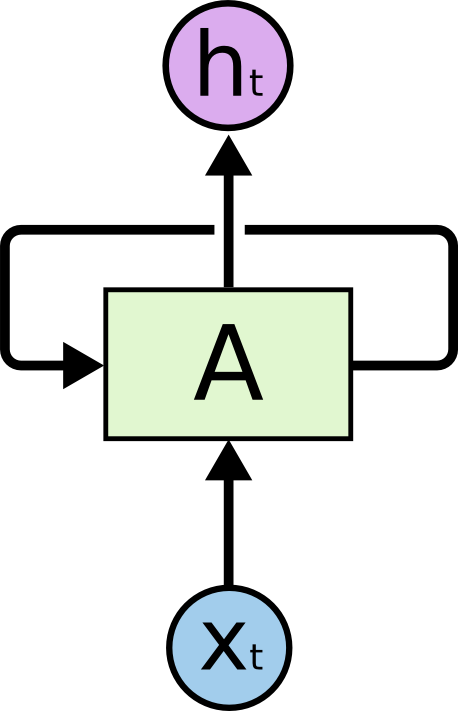
\includegraphics[scale=0.4]{./figs/rnn-rolled}
	\caption[A Rolled Recurrent Neural Networks]{Recurrent Neural Networks (RNNs) uses loops.}
	\label{fig:rnn-rolled}
\end{figure}

As it shown in \textbf{Figure \ref{fig:rnn-rolled}}, a selected neural network, $A$ takes the input $x_t$ and outputs the value of $h_t$. this might not show how data goes from one step to the next one in a same network until you unroll the loop and see chain architecture of recurrent neural networks that makes them the best choice for sequential data, \textbf{Figure \ref{fig:rnn-unrolled}}.

\begin{figure}[p]
	\centering
	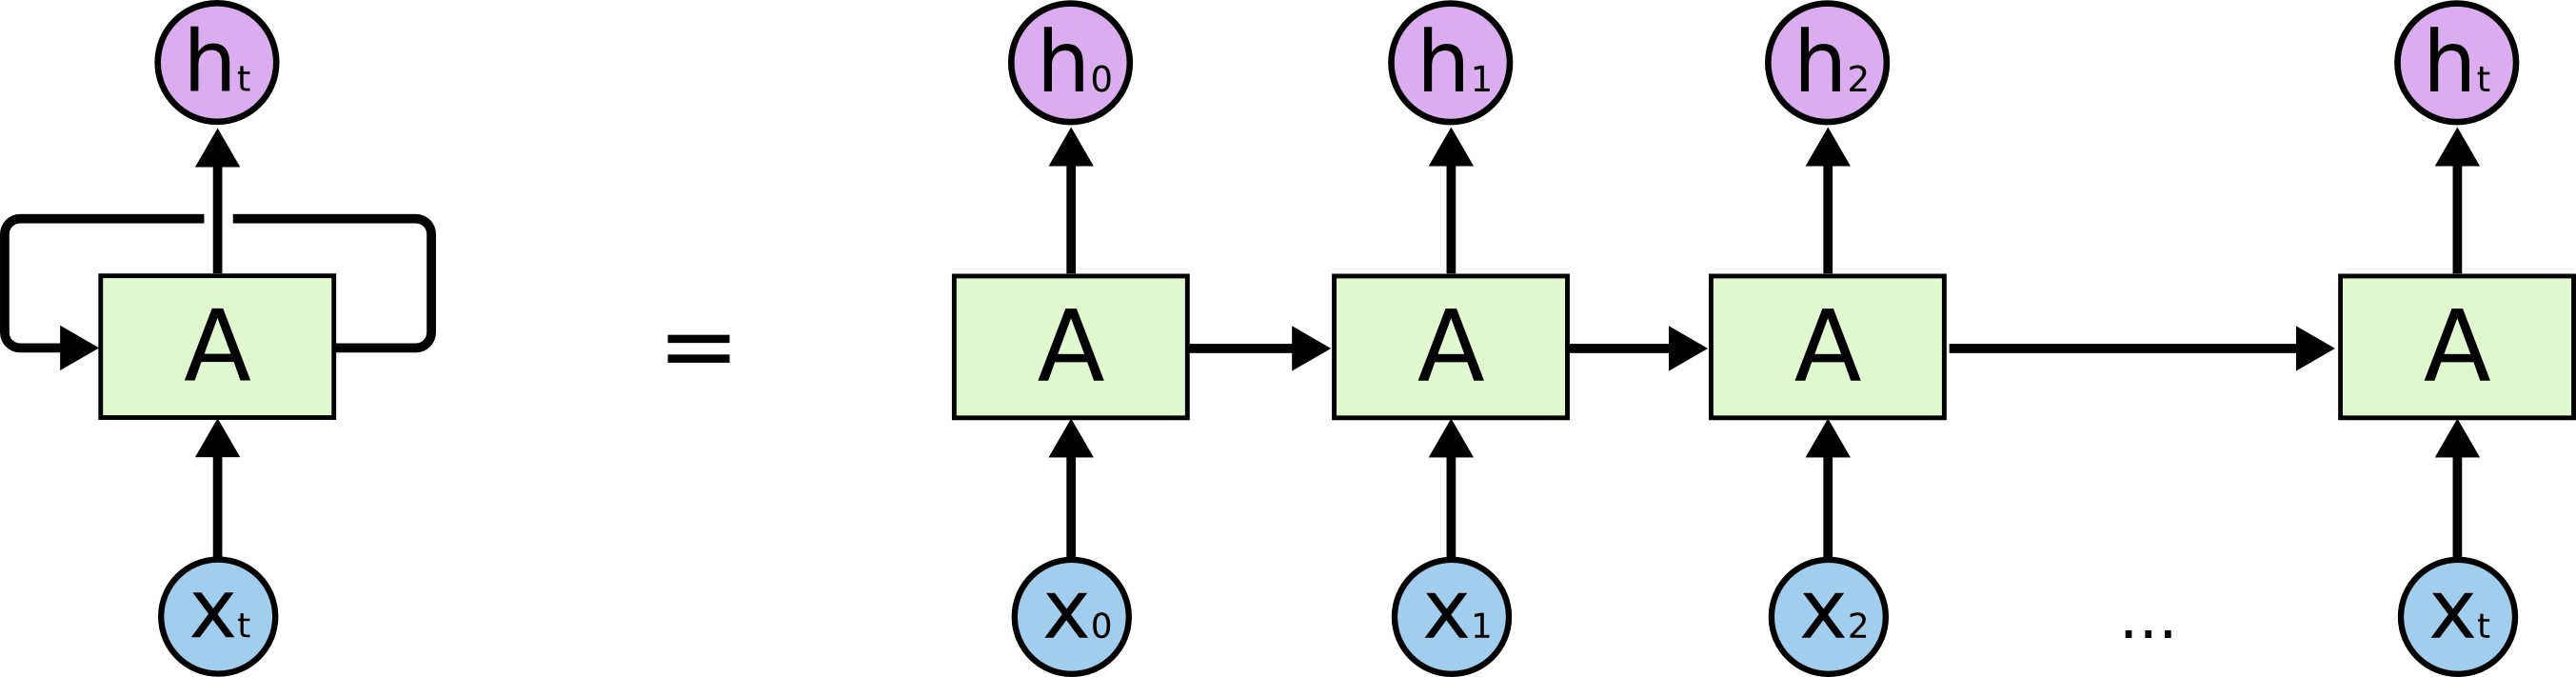
\includegraphics[scale=0.4]{./figs/rnn-unrolled}
	\caption[An Unrolled Recurrent Neural Networks]{An Unrolled Recurrent Neural Networks (RNNs).}
	\label{fig:rnn-unrolled}
\end{figure}

\subsection{Bayes by Backprop}

Bayes by Backprop \cite{Blundell2015a} is a variational inference scheme for learning the posterior distribution on the weights of a neural network.
The posterior distribution on parameters of the network $\theta \in \mathbb{R}^d$, $q(\theta)$ is typically taken to be a Gaussian with mean parameter $\mu\in \mathbb{R}^d$ and standard deviation parameter $\sigma\in \mathbb{R}^d$, denoted $\mathcal{N}(\theta|\mu,\sigma)$, noting that we use a diagonal covariance matrix, and where $d$ is the dimensionality of the parameters of the network (typically in the order of millions).
Let $\log p(y|\theta, x)$ be the log-likelihood of the neural network, then the
network is trained by minimising the variational free energy:
\begin{align}
	\label{eq:elbo}
	\mathcal{L}(\theta) &=
	\mathbb{E}_{q(\theta)}\left[\log \frac{q(\theta)}{p(y|\theta, x)p(\theta)}\right],
\end{align}
where $p(\theta)$ is a prior on the parameters.

Algorithm \ref{alg:bbb} shows the Bayes by Backprop Monte Carlo procedure for minimising \ref{eq:elbo} with respect to the mean and standard deviation parameters of the posterior $q(\theta)$.


Minimising the variational free energy \ref{eq:elbo} is equivalent to maximising the log-likelihood $\log p(y|\theta, x)$ subject to a KL complexity term on the parameters of the network that acts as a regulariser:
\begin{align}
	\label{eq:klelbo}
	\mathcal{L}(\theta) &=
	- \mathbb{E}_{q(\theta)}\left[\log p(y|\theta, x) \right]
	+ \kl{q(\theta)}{p(\theta)}.
\end{align}

In the Gaussian case with a zero mean prior, the KL term can be seen as a form of weight decay on the mean parameters, where the rate of weight decay is automatically tuned by the standard deviation parameters of the prior and posterior.


\begin{algorithm}[ht]
	\caption{Bayes by Backprop}
	\label{alg:bbb}
	\begin{algorithmic}
		\STATE{Sample $\epsilon \sim \mathcal{N}(0, I)$, $\epsilon \in \mathbb{R}^d$.}
		\STATE{Set network parameters to $\theta = \mu + \sigma\epsilon$.}
		\STATE{Do forward propagation and backpropagation as normal.}
		\STATE{Let $g$ be the gradient with respect	\label{eq:elbo}
			\mathcal{L}(\theta) &=
			\mathbb{E}_{q(\theta)}\left[\log \frac{q(\theta)}{p(y|\theta, x)p(\theta)}\right], to $\theta$ from backpropagation.} 
		\STATE{Let $g^{KL}_\theta, g^{KL}_\mu, g^{KL}_\sigma$ be the gradients of $\log \mathcal{N}(\theta|\mu, \sigma) - \log p(\theta)$ with respect to $\theta$, $\mu$ and 
			$\sigma$ respectively.} 
		\STATE{Update $\mu$ according to the gradient $g + g^{KL}_\theta + g^{KL}_\mu$.} 
		\STATE{Update $\sigma$ according to the gradient $(g + g^{KL}_\theta) \epsilon + g^{KL}_\sigma$.}
	\end{algorithmic}
\end{algorithm}

The uncertainty afforded by Bayes by Backprop trained networks has been used successfully for training feedforward models for supervised learning and to aid exploration by reinforcement learning agents \cite{Blundell2015a}, \cite{Lipton2016}, \cite{Houthooft2016}, but as yet, it has not been applied to recurrent neural networks.

\section{Backprop Through Time}
\label{sec:bptt}

The core of an RNN, $f$, is a neural network that maps the RNN state at step $t$, $s_t$ and an input observation $x_t$ to a new RNN state $s_{t+1}$, $f: (s_t, x_t) \mapsto s_{t+1}$.

For concreteness an LSTM core \cite{hochreiter1997long} has a state $s_t = (c_t, h_t)$ where $c$ is an internal core state and $h$ is the exposed state.
Intermediate gates modulate the effect of the inputs on the outputs, namely the input gate $i_t$, forget gate $f_t$ and output gate $o_t$.
The relationship between the inputs, outputs and internal gates of an LSTM cell (without peephole connections) are as follows:
\begin{align*}
i_t &= \sigma(W_i [x_t, h_{t-1}]^T + b_i), \\
f_t &= \sigma(W_f [x_t, h_{t-1}]^T + b_f), \\
c_t &= f_t c_{t-1} + i_t \tanh(W_c [x_t, h_{t-1}] + b_c), \\
o_t &= \sigma(W_o [x_t, h_{t-1}]^T + b_o), \\
h_t &= o_t \tanh(c_t),
\end{align*}
where $W_i$ ($b_i$), $W_f$ ($b_f$), $W_c$ ($b_c$) and $W_o$ ($b_o$) are the weights (biases) affecting the input gate, forget gate, cell update, and output gate respectively.

An RNN can be trained on a sequence of length $T$ by backpropagation through time where the RNN is unrolled $T$ times into a feedforward network.
That is, by forming the feedforward network with inputs
$x_1, x_2, \dots, x_T$ and initial state $s_0$:
\begin{align}
s_1 &= f(s_0, x_1), \nonumber \\
s_2 &= f(s_1, x_2), \nonumber \\
&\dots \nonumber \\
\label{eq:unroll}
s_T &= f(s_{T-1}, x_T), 
\end{align}
where $s_T$ is the final state of the RNN.
We shall refer to an RNN core unrolled for $T$ steps as in \eqref{eq:unroll} by $s_{1:T} = F_T(x_{1:T}, s_0)$,
where $x_{1:T}$ is the sequence of input vectors and $s_{1:T}$ is the sequence of corresponding states. Note that the truncated version of the algorithm can be seen as taking $s_0$ as the last state of the previous batch, $s_T$.

RNN parameters are learnt in much the same way as in a feedforward neural network.
A loss (typically after further layers) is applied to the states $s_{1:T}$ of the RNN, and then backpropagation is used to update the weights of the network.
Crucially, the weights at each of the unrolled step are shared. 
Thus each weight of the RNN core receives $T$ gradient contributions when the RNN is unrolled for $T$ steps.

\section{Truncated Bayes by Backprop Through Time}
\label{sec:tbbbtt}

Applying BBB to RNNs is depicted in Figure~\ref{fig:lstmbbb} where the weight matrices of the RNN are drawn from a distribution (learnt by BBB).
However, this direct application raises two questions: when to sample the parameters of the RNN, and how to weight the contribution of the KL regulariser of \eqref{eq:klelbo}.
We shall briefly justify the adaptation of BBB to RNNs, given in Algorithm~\ref{alg:rnnbbb} below.

\begin{figure}
	\centering
	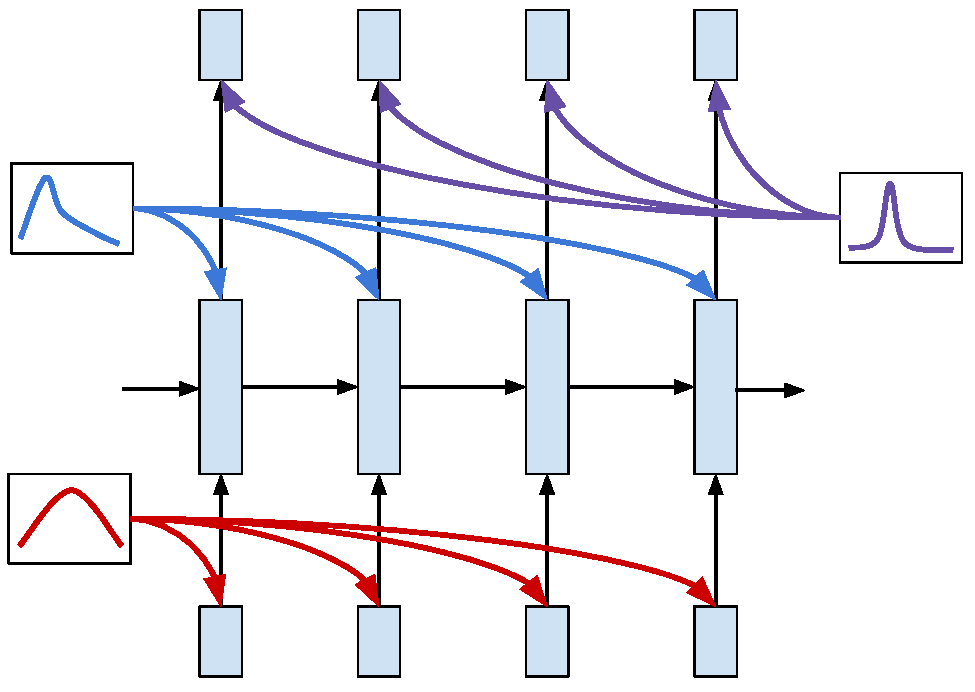
\includegraphics[width=\linewidth]{figs/LSTMBBB}
	\caption{Demonstration of Bayes by Backprop (BBB) applied to an RNN.}
	\label{fig:lstmbbb}
\end{figure}

The variational free energy of \eqref{eq:klelbo} for an RNN on a sequence of length $T$ is:
\begin{align}
\mathcal{L}(\theta) &=
- \mathbb{E}_{q(\theta)}\left[\log p(y_{1:T}|\theta, x_{1:T}) \right]
\nonumber \\
&\phantom{=}
+ \kl{q(\theta)}{p(\theta)},
\label{eq:rnnelbo}
\end{align}
where $p(y_{1:T}|\theta, x_{1:T})$ is the likelihood of a sequence produced when the states of an unrolled RNN $F_T$ are fed into an appropriate probability distribution.
The parameters of the entire network are $\theta$.
Although the RNN is unrolled $T$ times, each weight is penalised just once by the KL term, rather than $T$ times.
Also clear from \eqref{eq:rnnelbo} is that when a Monte Carlo approximation is taken to the expectation, the parameters $\theta$ should be held fixed throughout the entire sequence.

Two complications arise to the above naive derivation in practice: firstly, sequences are often long enough and models sufficiently large, that unrolling the RNN for the whole sequence is prohibitive.
Secondly, to reduce variance in the gradients, more than one sequence is trained at a time.
Thus the typical regime for training RNNs involves training on mini-batches of truncated sequences.

Let $B$ be the number of mini-batches and $C$ the number of truncated sequences (``cuts''),
then we can write \eqref{eq:rnnelbo} as:
\begin{align}
\mathcal{L}(\theta) &=
- \mathbb{E}_{q(\theta)}\left[\log \prod_{b=1}^B \prod_{c=1}^{C} p(y^{(b,c)}|\theta, x^{(b,c)}) \right]
\nonumber \\
&\phantom{=}
+ \kl{q(\theta)}{p(\theta)},
\end{align}
where the $(b,c)$ superscript denotes elements of $c$th truncated sequence in the $b$th minibatch.
Thus the free energy of mini-batch $b$ of a truncated sequence $c$ can be written as:
\begin{align}
\mathcal{L}_{(b,c)}(\theta) &=
- \mathbb{E}_{q(\theta)}\left[\log p(y^{(b,c)}|\theta, x^{(b,c)}, s^{(b,c)}_\text{prev}) \right]
\nonumber \\
&\phantom{=}
+ w^{(b,c)}_\text{KL} \kl{q(\theta)}{p(\theta)},
\label{eq:weightelbo}
\end{align}
where $w^{(b,c)}_\text{KL}$ distributes the responsibility of the KL cost among minibatches and truncated sequences (thus $\sum_{b=1}^B \sum_{c=1}^C w^{(b,c)}_\text{KL} = 1$), and $s^{(b,c)}_\text{prev}$ refers to the initial state of the RNN for the minibatch $x^{(b,c)}$.
In practice, we pick $w^{(b,c)}_\text{KL} = \frac{1}{C B}$ so that the KL penalty is equally distributed among all mini-batches and truncated sequences.
The truncated sequences in each subsequent mini-batches are picked in order, and so $s^{(b,c)}_\text{prev}$ is set to the last state of the RNN for $x^{(b,c-1)}$.

Finally, the question of when to sample weights follows naturally from taking a Monte Carlo approximations to \eqref{eq:weightelbo}: for each minibatch, sample a fresh set of parameters.

\begin{algorithm}[ht]
	\caption{Bayes by Backprop for RNNs}
	\label{alg:rnnbbb}
	\begin{algorithmic}
		\STATE{Sample $\epsilon \sim \mathcal{N}(0,I)$, $\epsilon \in \mathbb{R}^d$.}
		\STATE{Set network parameters to $\theta = \mu + \sigma\epsilon$.}
		\STATE{Sample a minibatch of truncated sequences $(x,y)$.}
		\STATE{Do forward propagation and backpropagation as normal on minibatch.}
		\STATE{Let $g$ be the gradient with respect to $\theta$ from backpropagation.}
		\STATE{Let $g^{KL}_\theta, g^{KL}_\mu, g^{KL}_\sigma$ be the gradients of $\log \mathcal{N}(\theta|\mu, \sigma) - \log p(\theta)$ w.r.t. $\theta$, $\mu$ and $\sigma$ respectively.}
		\STATE{Update $\mu$ according to the gradient $\frac{g + \frac{1}{C}g^{KL}_\theta}{B} + \frac{g^{KL}_\mu}{B C}$.}
		\STATE{Update $\sigma$ according to the gradient $\left(\frac{g + \frac{1}{C} g^{KL}_\theta}{B}\right) \epsilon + \frac{g^{KL}_\sigma}{B C}$.}
	\end{algorithmic}
\end{algorithm}

\subsection{Model Confidence}

\subsection{Model Uncertainty and Safety}

\section{State-of-the-Arts}

\section{Limitations}
\begin{enumerate}
\item Mentor~Graphics 2
\begin{enumerate}
\item item 3
\end{enumerate}
\item item 4
\end{enumerate}

\section{Research Gaps}
The processing at layer-5%
